\documentclass{book}
\usepackage[a4paper,top=2.5cm,bottom=2.5cm,left=2.5cm,right=2.5cm]{geometry}
\usepackage{makeidx}
\usepackage{natbib}
\usepackage{graphicx}
\usepackage{multicol}
\usepackage{float}
\usepackage{listings}
\usepackage{color}
\usepackage{ifthen}
\usepackage[table]{xcolor}
\usepackage{textcomp}
\usepackage{alltt}
\usepackage{ifpdf}
\ifpdf
\usepackage[pdftex,
            pagebackref=true,
            colorlinks=true,
            linkcolor=blue,
            unicode
           ]{hyperref}
\else
\usepackage[ps2pdf,
            pagebackref=true,
            colorlinks=true,
            linkcolor=blue,
            unicode
           ]{hyperref}
\usepackage{pspicture}
\fi
\usepackage[utf8]{inputenc}
\usepackage{mathptmx}
\usepackage[scaled=.90]{helvet}
\usepackage{courier}
\usepackage{sectsty}
\usepackage{amssymb}
\usepackage[titles]{tocloft}
\usepackage{doxygen}
\lstset{language=C++,inputencoding=utf8,basicstyle=\footnotesize,breaklines=true,breakatwhitespace=true,tabsize=4,numbers=left }
\makeindex
\setcounter{tocdepth}{3}
\renewcommand{\footrulewidth}{0.4pt}
\renewcommand{\familydefault}{\sfdefault}
\hfuzz=15pt
\setlength{\emergencystretch}{15pt}
\hbadness=750
\tolerance=750
\begin{document}
\hypersetup{pageanchor=false,citecolor=blue}
\begin{titlepage}
\vspace*{7cm}
\begin{center}
{\Large groogle \\[1ex]\large 1.\-0 }\\
\vspace*{1cm}
{\large Generated by Doxygen 1.8.3.1}\\
\vspace*{0.5cm}
{\small Sat Feb 2 2013 11:29:17}\\
\end{center}
\end{titlepage}
\clearemptydoublepage
\pagenumbering{roman}
\tableofcontents
\clearemptydoublepage
\pagenumbering{arabic}
\hypersetup{pageanchor=true,citecolor=blue}
\chapter{R\-E\-A\-D\-M\-E}
\label{md_README}
\hypertarget{md_README}{}
\input{md_README}
\chapter{Namespace Index}
\section{Namespace List}
Here is a list of all documented namespaces with brief descriptions\-:\begin{DoxyCompactList}
\item\contentsline{section}{\hyperlink{namespaceparser}{parser} }{\pageref{namespaceparser}}{}
\end{DoxyCompactList}

\chapter{Hierarchical Index}
\section{Class Hierarchy}
This inheritance list is sorted roughly, but not completely, alphabetically\-:\begin{DoxyCompactList}
\item \contentsline{section}{analyzer.\-Analyzer}{\pageref{classanalyzer_1_1Analyzer}}{}
\item \contentsline{section}{parser.\-Parser}{\pageref{classparser_1_1Parser}}{}
\item Q\-Graphics\-Item\begin{DoxyCompactList}
\item \contentsline{section}{link.\-Node}{\pageref{classlink_1_1Node}}{}
\item \contentsline{section}{node.\-Node}{\pageref{classnode_1_1Node}}{}
\end{DoxyCompactList}
\item Q\-Graphics\-Line\-Item\begin{DoxyCompactList}
\item \contentsline{section}{link.\-Link}{\pageref{classlink_1_1Link}}{}
\end{DoxyCompactList}
\item \contentsline{section}{query.\-Query}{\pageref{classquery_1_1Query}}{}
\item Q\-Widget\begin{DoxyCompactList}
\item \contentsline{section}{groogle\-View.\-Groogle\-View}{\pageref{classgroogleView_1_1GroogleView}}{}
\end{DoxyCompactList}
\item \contentsline{section}{scraper.\-Scraper}{\pageref{classscraper_1_1Scraper}}{}
\end{DoxyCompactList}

\chapter{Class Index}
\section{Class List}
Here are the classes, structs, unions and interfaces with brief descriptions\-:\begin{DoxyCompactList}
\item\contentsline{section}{\hyperlink{classanalyzer_1_1Analyzer}{analyzer.\-Analyzer} }{\pageref{classanalyzer_1_1Analyzer}}{}
\item\contentsline{section}{\hyperlink{classgroogleView_1_1GroogleView}{groogle\-View.\-Groogle\-View} }{\pageref{classgroogleView_1_1GroogleView}}{}
\item\contentsline{section}{\hyperlink{classlink_1_1Link}{link.\-Link} }{\pageref{classlink_1_1Link}}{}
\item\contentsline{section}{\hyperlink{classnode_1_1Node}{node.\-Node} }{\pageref{classnode_1_1Node}}{}
\item\contentsline{section}{\hyperlink{classlink_1_1Node}{link.\-Node} }{\pageref{classlink_1_1Node}}{}
\item\contentsline{section}{\hyperlink{classparser_1_1Parser}{parser.\-Parser} }{\pageref{classparser_1_1Parser}}{}
\item\contentsline{section}{\hyperlink{classquery_1_1Query}{query.\-Query} }{\pageref{classquery_1_1Query}}{}
\item\contentsline{section}{\hyperlink{classscraper_1_1Scraper}{scraper.\-Scraper} }{\pageref{classscraper_1_1Scraper}}{}
\end{DoxyCompactList}

\chapter{Namespace Documentation}
\hypertarget{namespaceparser}{\section{parser Namespace Reference}
\label{namespaceparser}\index{parser@{parser}}
}
\subsection*{Classes}
\begin{DoxyCompactItemize}
\item 
class \hyperlink{classparser_1_1Parser}{Parser}
\end{DoxyCompactItemize}
\subsection*{Functions}
\begin{DoxyCompactItemize}
\item 
def \hyperlink{namespaceparser_aadc91d7663f0db7213890c58651120d8}{main}
\end{DoxyCompactItemize}


\subsection{Detailed Description}
\begin{DoxyVerb}@package parser

The parser is used to take plain html and return the important words.

@note This really doesn't need to be used as a class, it's only used in a
      static context form.
\end{DoxyVerb}
 

\subsection{Function Documentation}
\hypertarget{namespaceparser_aadc91d7663f0db7213890c58651120d8}{\index{parser@{parser}!main@{main}}
\index{main@{main}!parser@{parser}}
\subsubsection[{main}]{\setlength{\rightskip}{0pt plus 5cm}def parser.\-main (
\begin{DoxyParamCaption}
{}
\end{DoxyParamCaption}
)}}\label{namespaceparser_aadc91d7663f0db7213890c58651120d8}
\begin{DoxyVerb}For testing purposes\end{DoxyVerb}
 
\chapter{Class Documentation}
\hypertarget{classanalyzer_1_1Analyzer}{\section{analyzer.\-Analyzer Class Reference}
\label{classanalyzer_1_1Analyzer}\index{analyzer.\-Analyzer@{analyzer.\-Analyzer}}
}
\subsection*{Public Member Functions}
\begin{DoxyCompactItemize}
\item 
\hypertarget{classanalyzer_1_1Analyzer_a3bfb8acf9d6b611543e51a4f7170ca27}{def {\bfseries \-\_\-\-\_\-init\-\_\-\-\_\-}}\label{classanalyzer_1_1Analyzer_a3bfb8acf9d6b611543e51a4f7170ca27}

\item 
\hypertarget{classanalyzer_1_1Analyzer_a69a08ee7b2a646b87f019d8b9553b853}{def {\bfseries combine\-Keywords}}\label{classanalyzer_1_1Analyzer_a69a08ee7b2a646b87f019d8b9553b853}

\item 
\hypertarget{classanalyzer_1_1Analyzer_afd09cd13d4b864f9df5d43c510759ab1}{def {\bfseries get\-Top\-Words}}\label{classanalyzer_1_1Analyzer_afd09cd13d4b864f9df5d43c510759ab1}

\item 
\hypertarget{classanalyzer_1_1Analyzer_af9a93d1bfcfc91e46ca2b1b2620d14c8}{def {\bfseries get\-Top\-Images}}\label{classanalyzer_1_1Analyzer_af9a93d1bfcfc91e46ca2b1b2620d14c8}

\item 
\hypertarget{classanalyzer_1_1Analyzer_aad1fd5c95914f1e660e33e2bbcc75798}{def {\bfseries get\-Top\-Videos}}\label{classanalyzer_1_1Analyzer_aad1fd5c95914f1e660e33e2bbcc75798}

\item 
\hypertarget{classanalyzer_1_1Analyzer_a14173ab2680c043c34bdbc89e7edc1d6}{def {\bfseries update\-View}}\label{classanalyzer_1_1Analyzer_a14173ab2680c043c34bdbc89e7edc1d6}

\end{DoxyCompactItemize}
\subsection*{Public Attributes}
\begin{DoxyCompactItemize}
\item 
\hypertarget{classanalyzer_1_1Analyzer_ae85923ff676fb1156a1c4dafd55d3213}{{\bfseries m\-Queries}}\label{classanalyzer_1_1Analyzer_ae85923ff676fb1156a1c4dafd55d3213}

\item 
\hypertarget{classanalyzer_1_1Analyzer_a383ed0736fdf320258645cf4c7a47f09}{{\bfseries m\-Keyword\-Hist}}\label{classanalyzer_1_1Analyzer_a383ed0736fdf320258645cf4c7a47f09}

\end{DoxyCompactItemize}


The documentation for this class was generated from the following file\-:\begin{DoxyCompactItemize}
\item 
analyzer.\-py\end{DoxyCompactItemize}

\hypertarget{classview_1_1Example}{\section{view.\-Example Class Reference}
\label{classview_1_1Example}\index{view.\-Example@{view.\-Example}}
}
Inheritance diagram for view.\-Example\-:\begin{figure}[H]
\begin{center}
\leavevmode
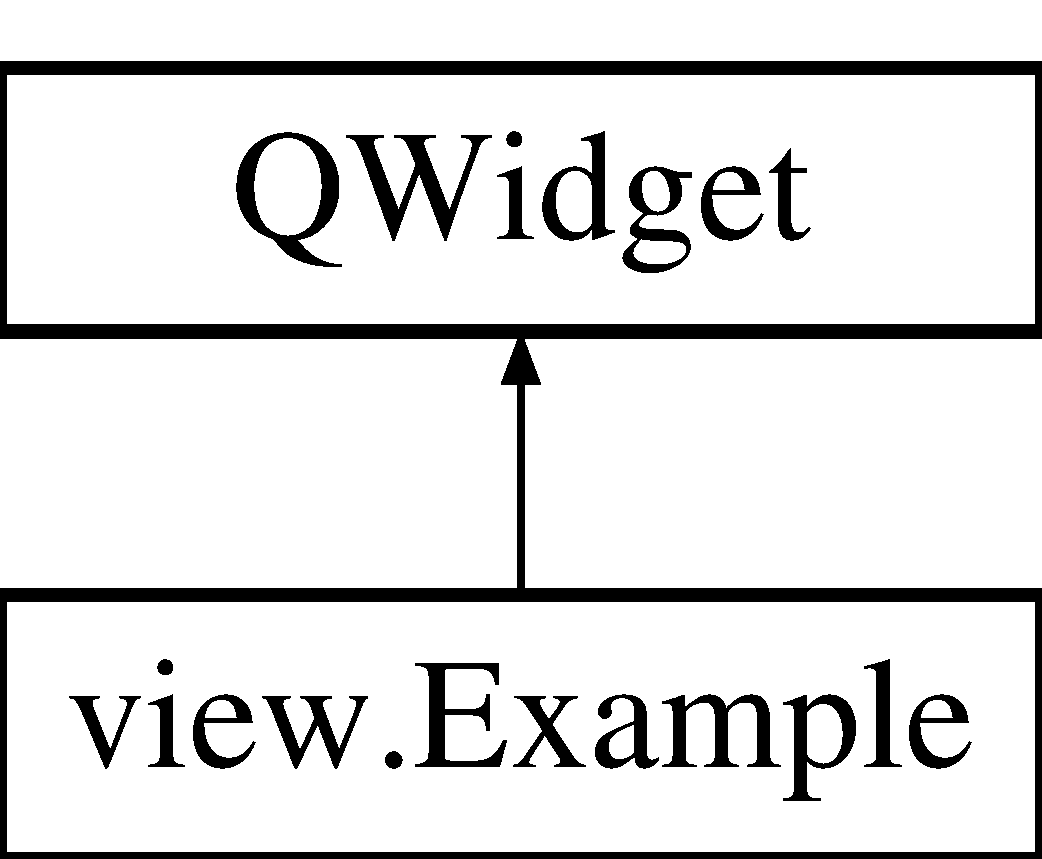
\includegraphics[height=2.000000cm]{classview_1_1Example}
\end{center}
\end{figure}
\subsection*{Public Member Functions}
\begin{DoxyCompactItemize}
\item 
\hypertarget{classview_1_1Example_ab71d851c4701b16b75f5b07d7e299dbd}{def {\bfseries \-\_\-\-\_\-init\-\_\-\-\_\-}}\label{classview_1_1Example_ab71d851c4701b16b75f5b07d7e299dbd}

\item 
\hypertarget{classview_1_1Example_a18cfda95cbf601790d1020c3bf3f83fb}{def {\bfseries init\-U\-I}}\label{classview_1_1Example_a18cfda95cbf601790d1020c3bf3f83fb}

\item 
\hypertarget{classview_1_1Example_ae4f51d4c6190cf041a32f5ef47a02912}{def {\bfseries add\-Node}}\label{classview_1_1Example_ae4f51d4c6190cf041a32f5ef47a02912}

\item 
\hypertarget{classview_1_1Example_a09ecb51e66e624bcf7453e54aecea55d}{def {\bfseries draw\-Rectangles}}\label{classview_1_1Example_a09ecb51e66e624bcf7453e54aecea55d}

\end{DoxyCompactItemize}
\subsection*{Public Attributes}
\begin{DoxyCompactItemize}
\item 
\hypertarget{classview_1_1Example_a593d2f15ead06099bd90e4c1523f9af2}{{\bfseries m\-Scene}}\label{classview_1_1Example_a593d2f15ead06099bd90e4c1523f9af2}

\item 
\hypertarget{classview_1_1Example_a77cbbbc9c24ea48834b0cbc4ee70cd44}{{\bfseries m\-View}}\label{classview_1_1Example_a77cbbbc9c24ea48834b0cbc4ee70cd44}

\item 
\hypertarget{classview_1_1Example_adc6ad20992e91847c2eca453a2e48e80}{{\bfseries m\-Nodes}}\label{classview_1_1Example_adc6ad20992e91847c2eca453a2e48e80}

\item 
\hypertarget{classview_1_1Example_a1aedee1f1cd91ca85b5baca3c4925d87}{{\bfseries m\-Links}}\label{classview_1_1Example_a1aedee1f1cd91ca85b5baca3c4925d87}

\end{DoxyCompactItemize}


The documentation for this class was generated from the following file\-:\begin{DoxyCompactItemize}
\item 
view.\-py\end{DoxyCompactItemize}

\hypertarget{classparser_1_1Parser}{\section{parser.\-Parser Class Reference}
\label{classparser_1_1Parser}\index{parser.\-Parser@{parser.\-Parser}}
}
\subsection*{Public Member Functions}
\begin{DoxyCompactItemize}
\item 
\hypertarget{classparser_1_1Parser_a970813fabceef8e022be33279f564ce8}{def {\bfseries \-\_\-\-\_\-init\-\_\-\-\_\-}}\label{classparser_1_1Parser_a970813fabceef8e022be33279f564ce8}

\item 
def \hyperlink{classparser_1_1Parser_a56a4ab5316fea1a523fbd9378f517650}{parse}
\item 
\hypertarget{classparser_1_1Parser_a0295c9dfc60bc342b26afb05f095ea96}{def {\bfseries clean\-H\-T\-M\-L}}\label{classparser_1_1Parser_a0295c9dfc60bc342b26afb05f095ea96}

\item 
\hypertarget{classparser_1_1Parser_a598633d4b01ba904f0154fa19826c384}{def {\bfseries select\-N\-L\-T\-K\-Nouns}}\label{classparser_1_1Parser_a598633d4b01ba904f0154fa19826c384}

\item 
\hypertarget{classparser_1_1Parser_aeb28313317dd1ed5af1631813641d170}{def {\bfseries remove\-Dirty\-Contains}}\label{classparser_1_1Parser_aeb28313317dd1ed5af1631813641d170}

\item 
\hypertarget{classparser_1_1Parser_ac7a3790160a8f661c6c08123a0aa1718}{def {\bfseries remove\-Dirty\-Words}}\label{classparser_1_1Parser_ac7a3790160a8f661c6c08123a0aa1718}

\end{DoxyCompactItemize}
\subsection*{Public Attributes}
\begin{DoxyCompactItemize}
\item 
\hypertarget{classparser_1_1Parser_a4037b5d92197b949f9728de47a754b16}{{\bfseries nouns}}\label{classparser_1_1Parser_a4037b5d92197b949f9728de47a754b16}

\item 
\hypertarget{classparser_1_1Parser_ac3cc5b6a9f0e1e383b8ba8eba92a9d56}{{\bfseries m\-Noun\-Hist}}\label{classparser_1_1Parser_ac3cc5b6a9f0e1e383b8ba8eba92a9d56}

\end{DoxyCompactItemize}


\subsection{Member Function Documentation}
\hypertarget{classparser_1_1Parser_a56a4ab5316fea1a523fbd9378f517650}{\index{parser\-::\-Parser@{parser\-::\-Parser}!parse@{parse}}
\index{parse@{parse}!parser::Parser@{parser\-::\-Parser}}
\subsubsection[{parse}]{\setlength{\rightskip}{0pt plus 5cm}def parser.\-Parser.\-parse (
\begin{DoxyParamCaption}
\item[{}]{self, }
\item[{}]{words}
\end{DoxyParamCaption}
)}}\label{classparser_1_1Parser_a56a4ab5316fea1a523fbd9378f517650}
\begin{DoxyVerb}Main parser function for parser class, removes all the cluter, and returns
all the important words.

@param words Single string of html
@retval Histogram in the form { word(string) : count (int) }
\end{DoxyVerb}
 

The documentation for this class was generated from the following file\-:\begin{DoxyCompactItemize}
\item 
parser.\-py\end{DoxyCompactItemize}

\hypertarget{classquery_1_1Query}{\section{query.\-Query Class Reference}
\label{classquery_1_1Query}\index{query.\-Query@{query.\-Query}}
}
\subsection*{Public Member Functions}
\begin{DoxyCompactItemize}
\item 
\hypertarget{classquery_1_1Query_a03c16181d9ce65cb7264b029b432fe7b}{def {\bfseries \-\_\-\-\_\-init\-\_\-\-\_\-}}\label{classquery_1_1Query_a03c16181d9ce65cb7264b029b432fe7b}

\item 
\hypertarget{classquery_1_1Query_ac58e18c6ba0209b084cb24c0dd9f2b3a}{def {\bfseries \-\_\-\-\_\-str\-\_\-\-\_\-}}\label{classquery_1_1Query_ac58e18c6ba0209b084cb24c0dd9f2b3a}

\end{DoxyCompactItemize}
\subsection*{Public Attributes}
\begin{DoxyCompactItemize}
\item 
\hypertarget{classquery_1_1Query_a3067f8805d7e11ba99dd6c8b47387460}{{\bfseries m\-Title}}\label{classquery_1_1Query_a3067f8805d7e11ba99dd6c8b47387460}

\item 
\hypertarget{classquery_1_1Query_af9e17a3a3f5284c0f2eedd8b4f1758da}{{\bfseries m\-U\-R\-L}}\label{classquery_1_1Query_af9e17a3a3f5284c0f2eedd8b4f1758da}

\item 
\hypertarget{classquery_1_1Query_a29cc3b88d60442b84745e21a8a1cd504}{{\bfseries m\-Image\-U\-R\-Ls}}\label{classquery_1_1Query_a29cc3b88d60442b84745e21a8a1cd504}

\item 
\hypertarget{classquery_1_1Query_a8d685c4ef0df5faafaec1b1284f00c38}{{\bfseries m\-Video\-U\-R\-Ls}}\label{classquery_1_1Query_a8d685c4ef0df5faafaec1b1284f00c38}

\item 
\hypertarget{classquery_1_1Query_af6497f231f86376ecb130d2c3248c38b}{{\bfseries m\-H\-T\-M\-L\-U\-R\-Ls}}\label{classquery_1_1Query_af6497f231f86376ecb130d2c3248c38b}

\item 
\hypertarget{classquery_1_1Query_a9b1607519ffb10c67a2f68b747853d87}{{\bfseries m\-Keyword\-Hist}}\label{classquery_1_1Query_a9b1607519ffb10c67a2f68b747853d87}

\item 
\hypertarget{classquery_1_1Query_a827264b4b6ded1a8b6b1d917d3daed5e}{{\bfseries m\-Google\-Query}}\label{classquery_1_1Query_a827264b4b6ded1a8b6b1d917d3daed5e}

\item 
\hypertarget{classquery_1_1Query_a8b312c607fd79c3ddd3968cb44cd59cd}{{\bfseries m\-Depth}}\label{classquery_1_1Query_a8b312c607fd79c3ddd3968cb44cd59cd}

\item 
\hypertarget{classquery_1_1Query_adbd462b8bd021032a8d19439e5eb52d5}{{\bfseries m\-H\-T\-M\-L}}\label{classquery_1_1Query_adbd462b8bd021032a8d19439e5eb52d5}

\end{DoxyCompactItemize}


The documentation for this class was generated from the following file\-:\begin{DoxyCompactItemize}
\item 
query.\-py\end{DoxyCompactItemize}

\hypertarget{classscraper_1_1Scraper}{\section{scraper.\-Scraper Class Reference}
\label{classscraper_1_1Scraper}\index{scraper.\-Scraper@{scraper.\-Scraper}}
}
\subsection*{Public Member Functions}
\begin{DoxyCompactItemize}
\item 
\hypertarget{classscraper_1_1Scraper_aab2046c61d81f97f4ca91f5d82a3e93b}{def {\bfseries \-\_\-\-\_\-init\-\_\-\-\_\-}}\label{classscraper_1_1Scraper_aab2046c61d81f97f4ca91f5d82a3e93b}

\item 
\hypertarget{classscraper_1_1Scraper_a1e363cf9112a9fab5c0de49b65a60ecf}{def {\bfseries get\-Title}}\label{classscraper_1_1Scraper_a1e363cf9112a9fab5c0de49b65a60ecf}

\item 
\hypertarget{classscraper_1_1Scraper_aa930865ef6567c2b8daf29295a9b61f5}{def {\bfseries get\-Html}}\label{classscraper_1_1Scraper_aa930865ef6567c2b8daf29295a9b61f5}

\item 
\hypertarget{classscraper_1_1Scraper_a83d540593a1fc58851432ad83b12992c}{def {\bfseries get\-Links}}\label{classscraper_1_1Scraper_a83d540593a1fc58851432ad83b12992c}

\item 
\hypertarget{classscraper_1_1Scraper_af9b594f2792b57580d7bc5aac581e85c}{def {\bfseries get\-Image\-Links}}\label{classscraper_1_1Scraper_af9b594f2792b57580d7bc5aac581e85c}

\item 
\hypertarget{classscraper_1_1Scraper_a1e5e5e16c03a9ee6709ed10da0dc75a1}{def {\bfseries scrape\-All}}\label{classscraper_1_1Scraper_a1e5e5e16c03a9ee6709ed10da0dc75a1}

\end{DoxyCompactItemize}
\subsection*{Public Attributes}
\begin{DoxyCompactItemize}
\item 
\hypertarget{classscraper_1_1Scraper_a29f1b1abf2adaea2fe782622748a00df}{{\bfseries m\-Br}}\label{classscraper_1_1Scraper_a29f1b1abf2adaea2fe782622748a00df}

\item 
\hypertarget{classscraper_1_1Scraper_a72e792b3ed75c00315b515da29244a37}{{\bfseries is\-Bad}}\label{classscraper_1_1Scraper_a72e792b3ed75c00315b515da29244a37}

\item 
\hypertarget{classscraper_1_1Scraper_ac5b7229df7b2f0589ea1fe8651e71cc1}{{\bfseries m\-H\-T\-M\-L}}\label{classscraper_1_1Scraper_ac5b7229df7b2f0589ea1fe8651e71cc1}

\item 
\hypertarget{classscraper_1_1Scraper_a97c7efed94f7b2119db66b52cc749457}{{\bfseries m\-Soup}}\label{classscraper_1_1Scraper_a97c7efed94f7b2119db66b52cc749457}

\end{DoxyCompactItemize}


The documentation for this class was generated from the following file\-:\begin{DoxyCompactItemize}
\item 
scraper.\-py\end{DoxyCompactItemize}

\addcontentsline{toc}{part}{Index}
\printindex
\end{document}
